\chapter{基础程序与输出}
\begin{introduction}
	\item hello world
	\item cout
	\item cin
	\item endl
	\item online judge
	\item 洛谷
\end{introduction}

\section{第一个程序}
在前面安装软件的过程中,我们使用了一段程序代码来测试集成开发环境是否安装成功,接下来我们解释一下各个代码语句的作用。

\begin{minted}{C++}
#include <iostream>
using namespace std;
int main()
{
	cout<<"Hello world";
	return 0;
}
\end{minted}

对于第一行代码\texttt{\#include <iostream>},作用是引入头文件。举例理解下这一行代码的作用,我们去上手工课,例如需要去剪纸,我们需要一些工具如剪刀、纸张等工具才能完成剪纸这个任务。头文件可以理解为一个仓库,里面就放着各种各样的工具供我们使用。

这次使用的 \texttt{iostream}头文件里面就包含了很多与输入输出有关的工具。后面我们还会接触到更多的头文件,会包含不同功能的工具。

对于第二行代码\texttt{using namespace std;},作用是使用命名空间。举例理解下这一行代码的作用,在教室中,突然广播中传来了教务主任的声音“请王小明同学来教务处一趟。”这个时候会存在这样一个问题,可能一年级一班有个叫王小明的同学,三年级八班也有个叫王小明的同学,光是通知名字的话,出现了重名是没有办法确认是叫哪个同学的。程序当中也是一样,可能会存在同名的工具,但是功能是不一样的。此时为了明确信息,生活中我们可以加上具体的来源信息,比如让三年级八班的王小明去一趟教务处。程序当中也是一样,通过命名空间告诉计算机从哪个地方去找对应名字的工具。

对于第三行代码\texttt{int main()},它是主函数,是程序的执行的入口,后面对应的\texttt{return 0;}是程序的出口。可以发现,\texttt{int main()}后面跟了一对大括号\texttt{\{\}},大括号里面就是我们初期学习时,书写代码的地方。

在这里,我们额外介绍一个叫做注释的东西,注释可以理解为我们的笔记,记录我们对内容的解释和说明,有两种注释方式,一种是单行注释,另一种是多行注释。
\begin{minted}{C++}
// 单行注释
/*
多
行
注
释
*/
\end{minted}
我们给程序的基本框架加上注释,这个框架希望同学们能记忆、背诵下来,以后我们的程序都是在这个框架上实现的。
\begin{mbdm}
\begin{minted}{C++}
#include <iostream> //引入头文件
using namespace std;//使用命名空间
int main()          //主函数,程序入口
{
	/*
	代
	码
	书
	写
	区
	域
	*/
	return 0;       //返回值,程序出口
}
\end{minted}
\end{mbdm}
第一个程序的第五行\texttt{cout<<"Hello world";}是输出语句,是用于让计算机呈现一些内容的。进行输出的话,我们需要用到一个工具\texttt{cout},使用方法如下:
\begin{minted}{C++}
cout<<"输出内容";
\end{minted}
\texttt{cout}可以视为为\textbf{c}omputer \textbf{out}put,也就是计算机输出,这样容易记忆些。双引号里面为输出内容,你写在里面的内容,计算机会原封不动地输出在屏幕上。

介绍完第一个程序的代码作用后,我们现在来尝试动手写一下,并运行一下,查看一下效果。第一个程序大家可以参考之前的代码,学习新东西,我们先从模仿开始。

在实现过程中,大家可能会遇到各种各样的问题,我们简单说几个容易犯的错误,大家自己注意下:
\begin{enumerate}
\item 输入法切换为\textbf{英文}输入状态。程序中所有的符号和都在英文状态下进行输入。
\item 每个语句的结束,需要加上分号\texttt{;},对应语句的结束。
\item 语句书写不要拼写错误,请仔细检查。
\end{enumerate}

\section{利用OJ辅助学习}
很多时候,当我们学习了一个知识点后,需要知道自己对该知识点的掌握情况,数学学习中可以通过练习册与对应的参考答案来进行检测。那么信息学竞赛的学习又该如何进行检测呢,一道题目,可能有多种实现的方式、多种不同的情况又该如何进行代码的评价?在线测评系统(Online Judge)正好能解决这样的痛点,本书的例题、练习也会利用这些在线测评系统进行,主要是在洛谷\footnote{洛谷在线题库,www.luogu.com.cn}、HDU\footnote{杭州电子科技大学在线题库,acm.hdu.edu.cn}和POJ\footnote{北京大学在线题库,poj.orj}上。

以洛谷B2002 Hello,World!一题为例,讲解下OJ的基础使用方式。在此之前请同学们先在网站上注册好帐号。

进入首页后,在问题跳转处输入题号,点击跳转,即可跳转到对应的题目。或者点击左边栏的题库,在关键词中进行搜索题号或题目名字。

% TODO: \usepackage{graphicx} required
\begin{figure}[H]
\centering
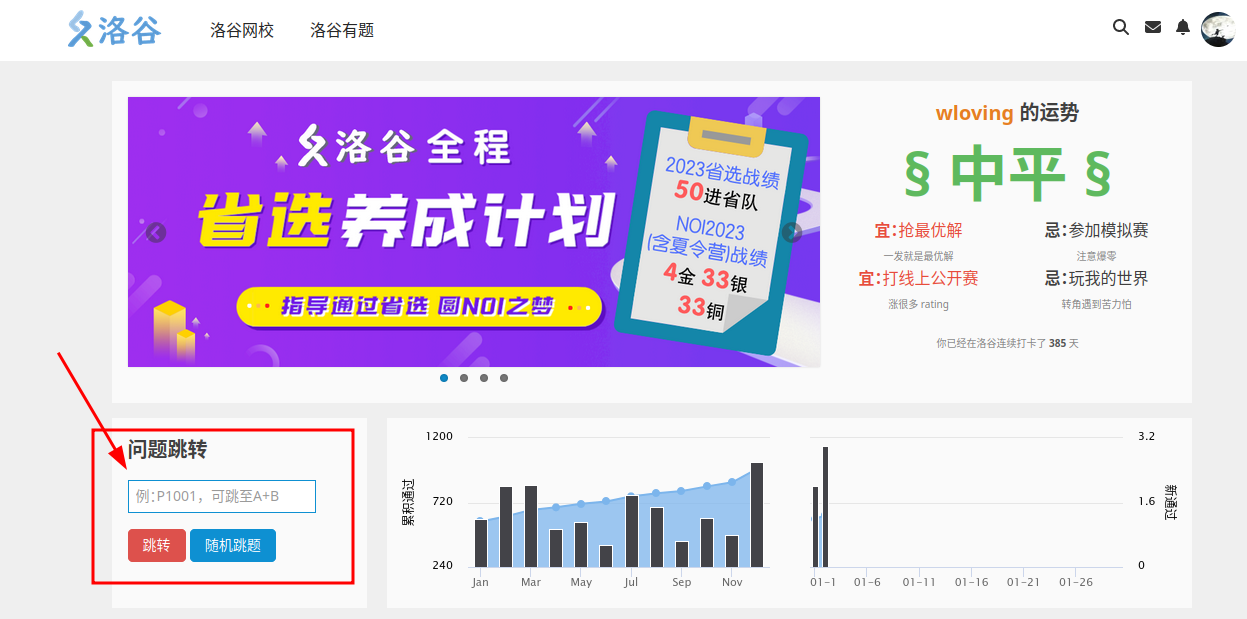
\includegraphics[width=0.4\linewidth]{02chapter/img/问题跳转}
\hspace{1in}
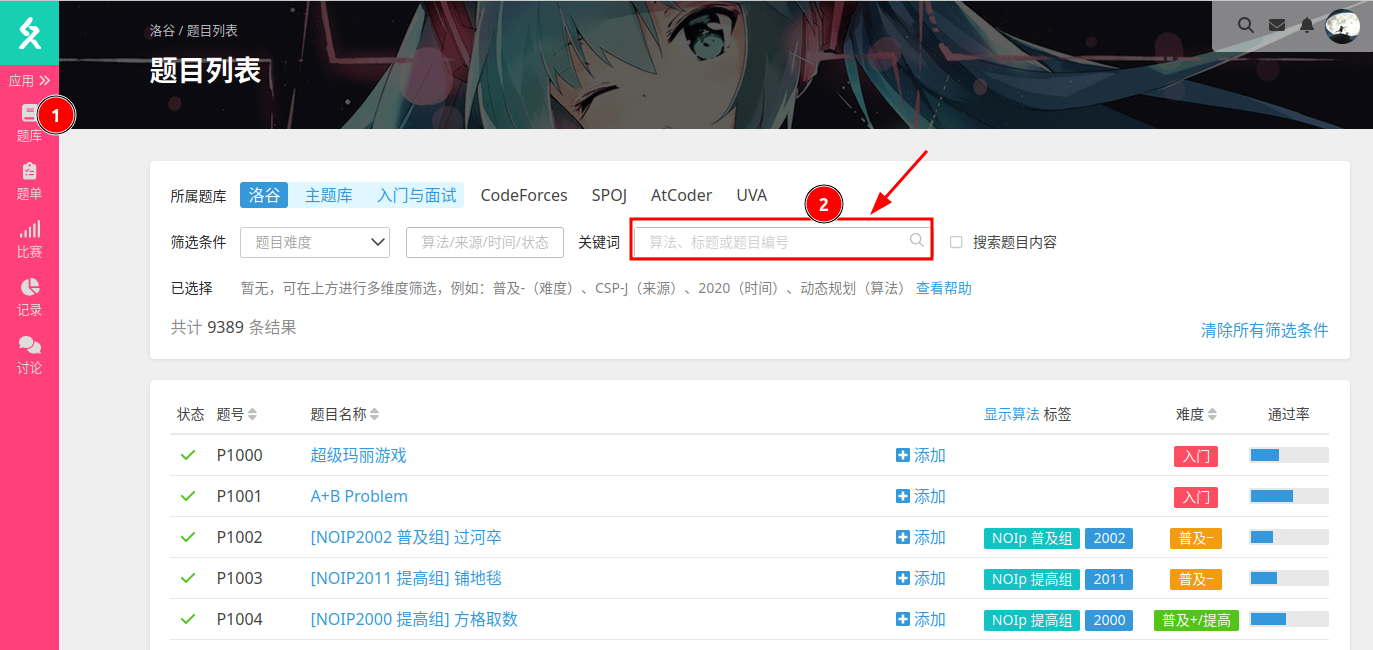
\includegraphics[width=0.4\linewidth]{02chapter/img/题库}
\caption{OJ搜题}
\label{fig:}
\end{figure}

进入题目后,点击左上角蓝色的提交答案按钮,在文本框中复制粘贴你写的代码,并点击左下角红色提交测评按钮,稍等片刻即可返回测评结果。
% TODO: \usepackage{graphicx} required
\begin{figure}[H]
\centering
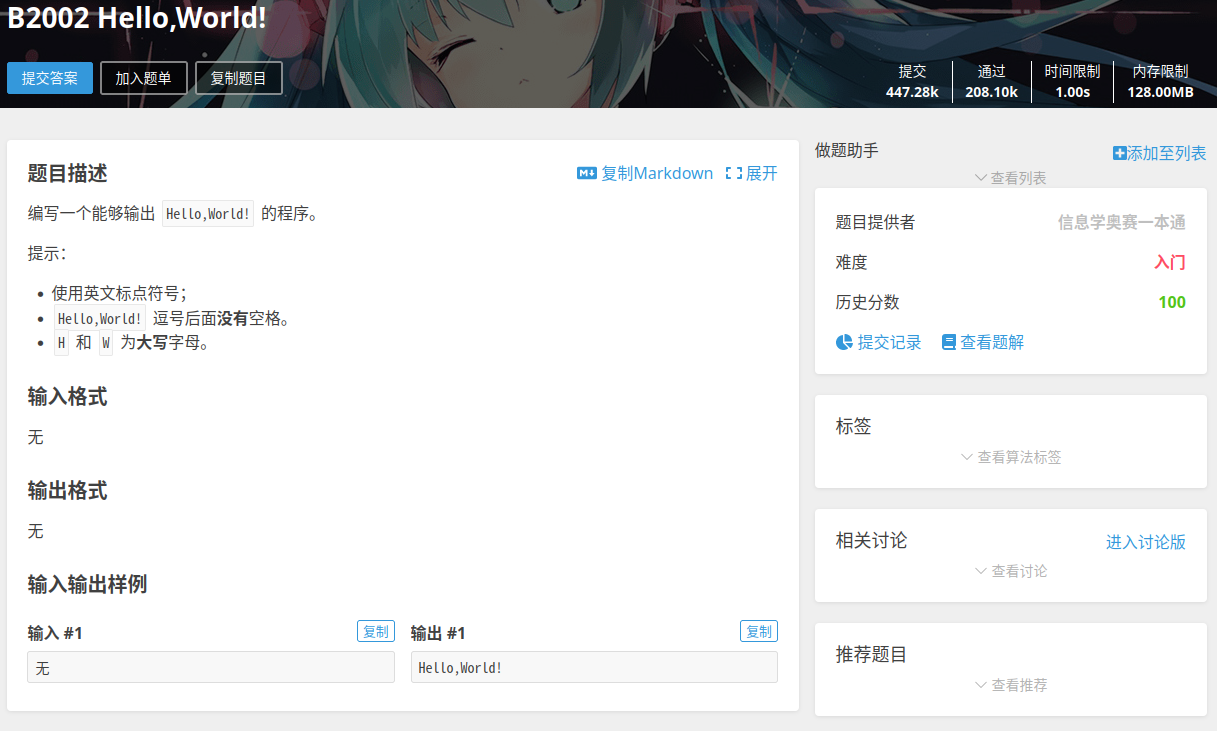
\includegraphics[width=0.4\linewidth]{02chapter/img/题面信息}
\hspace{1in}
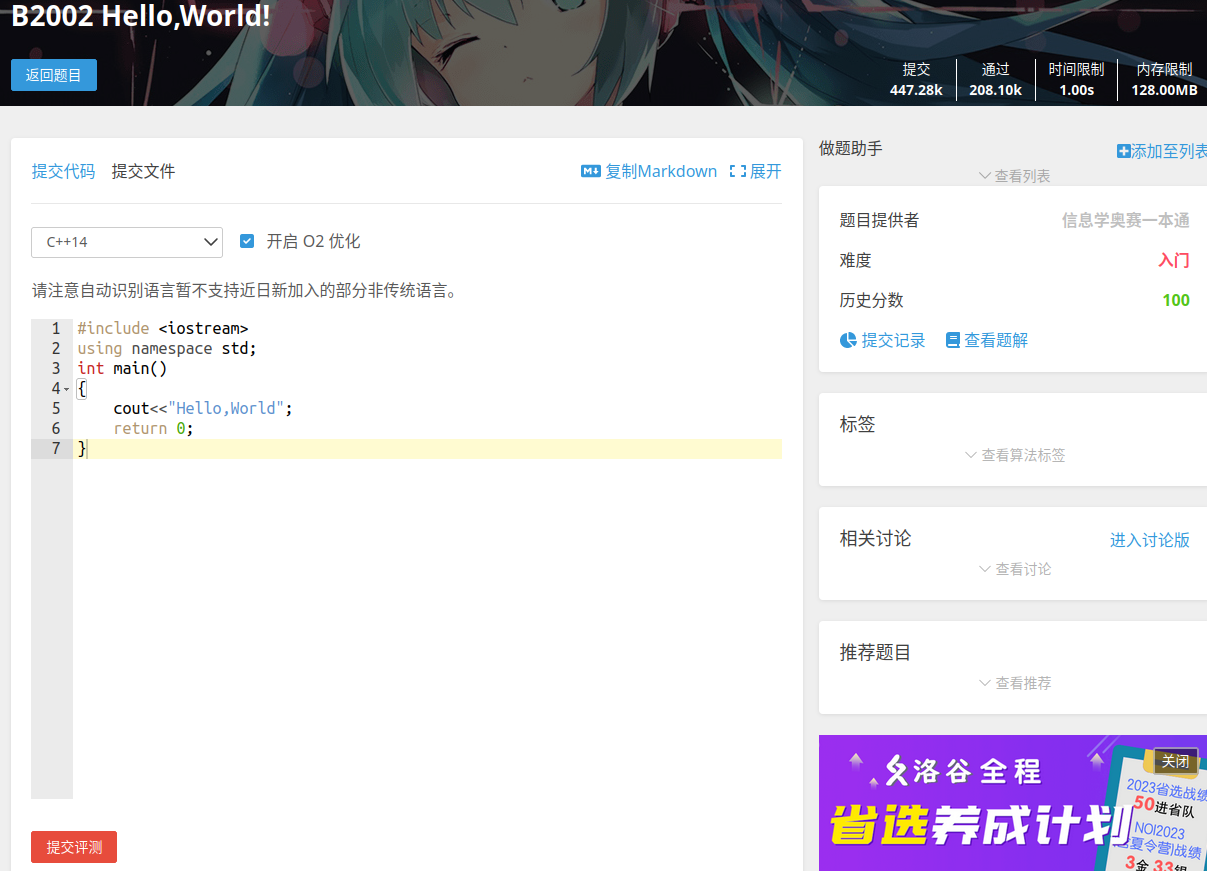
\includegraphics[width=0.4\linewidth]{02chapter/img/提交测评}
\caption{提交测评}
\label{fig:}
\end{figure}
对于测评结果会出现以下几种常见的情况。
\begin{enumerate}
\item \textcolor[RGB]{52,152,219}{Waiting/Juding/Pending}:程序正在等待测评或者正在测评。
\item \textcolor[RGB]{82,196,26}{Accepted(AC)}:程序通过了测试点。
\item \textcolor[RGB]{250,219,20}{Compile Error(CE)}:程序编译错误。
\item \textcolor[RGB]{231,76,60}{Wrong Answer(WA)}:错误的答案。
\item \textcolor[RGB]{157,61,207}{Runtime Error(RE)}:运行时错误。
\item \textcolor[RGB]{5,34,66}{Time Limit Exceeded(TLE)}:超出时间限制。
\item \textcolor[RGB]{5,34,66}{Memory Limit Exceeded(MLE)}:超出内存限制。
\end{enumerate}

大家可以尝试在洛谷OJ上完成一下\textbf{B2002 Helli,World!}这道题目。
\begin{dmsx}
\begin{minted}{C++}
#include <iostream>//引入头文件
using namespace std;//使用命名空间
int main()//主函数,程序入口
{
	cout<<"Hello,World!";//输出格式cout<<"输出内容";
	return 0;//程序出口
}

\end{minted}
\end{dmsx}

\section{输出的格式要求}
在测评时,我们要求自己写的程序输出格式需要与程序的输出格式要求保持一致,常见的一个输出格式要求就是换行,将多个内容换行输出。此时若仅是在源代码中将语句分行书写并无法达成换行的效果,可以通过以下的两种方法来实现换行。
\subsection{\texttt{endl}}
\begin{minted}{C++}
#include <iostream>//引入头文件
using namespace std;//使用命名空间
int main()//主函数,程序入口
{
	cout<<"Hello,World!"<<endl;//通过endl进行换行
	cout<<"Hello,World!";
	return 0;//程序出口
}
\end{minted}
多段内容用一个\texttt{cout}进行输出时,可以使用\texttt{<<}符号进行内容的链接。
\subsection{\texttt{$\backslash$n}}
\begin{minted}{C++}
#include <iostream>//引入头文件
using namespace std;//使用命名空间
int main()//主函数,程序入口
{
	cout<<"Hello,World!\n";//通过\n进行换行
	cout<<"Hello,World!";
	return 0;//程序出口
}
\end{minted}
\texttt{$\backslash$n}为转义字符,起换行的作用。
\subsection{输出字符菱形}
用\texttt{*}造一个对角线长 $5$ 个字符,倾斜放置的菱形。
\begin{minted}{text}
  *
 ***
*****
 ***
  *
\end{minted}

本题为洛谷B2025,大家可以结合刚刚补充的换行的知识,尝试完成一下这道题目。
\begin{tmfx}
题目要求很直接,要求仿照给的图形进行输出。

仔细观察每一行的内容。第1行为2个空格加1个\texttt{*}。第2行是1个空格加3个\texttt{*}。第3行是0个空格加5个\texttt{*}。第4行是1个空格加3个\texttt{*}。第5行是2个空格加1个\texttt{*}。

也可以不用去数,直接复制粘贴给出图案中的内容,放入\texttt{cout<<"输出内容"<<endl;}的结构中。
\end{tmfx}
\begin{dmsx}
\begin{minted}{C++}
#include <iostream>
using namespace std;
int main()
{
	cout<<"  *"<<endl;
	cout<<" ***"<<endl;
	cout<<"*****"<<endl;
	cout<<" ***"<<endl;
	cout<<"  *";
	return 0;
}
\end{minted}
\end{dmsx}
在进行多行内容书写时,大家要注意代码的风格,主函数中的代码不要定格书写,利用\texttt{Tab}制表符进行对齐,让程序具有层次感,便于我们进行阅读、复习。
\begin{problemset}
\item 洛谷B2002 Hello,World!
\item 洛谷B2025 输出字符菱形
\item 洛谷P1000 超级玛丽游戏
\end{problemset}


